\textbf{Notes} Procedures denoted in boldface, as separate sections.\\
\emph{n-D} does not include time\\
Refs \cite{sciplan} in exc.bib

\subsection{Base classes}\label{sec:base-classes}
The proposed base classes for \nep\ are listed below and shown graphically in \Fig{baseclasses}.
\begin{figure}
\centerline{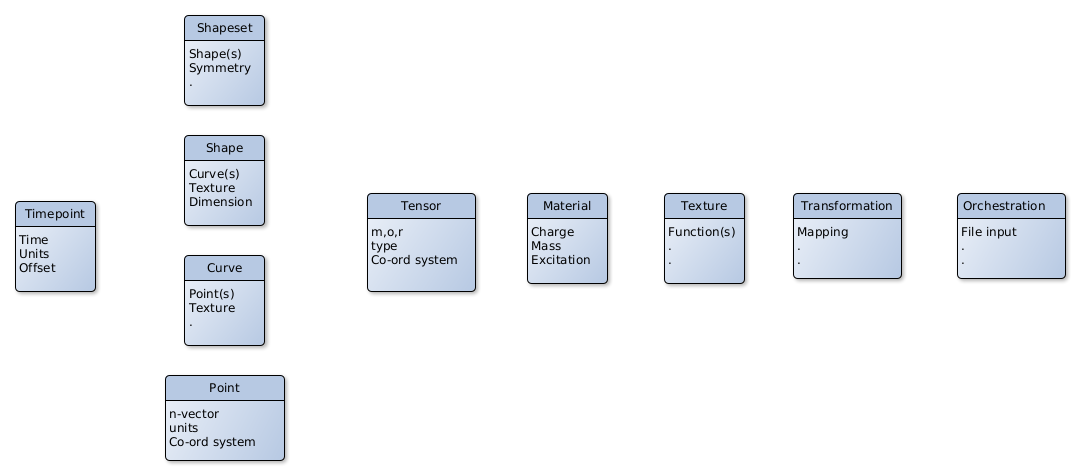
\includegraphics[width=0.7\textwidth]{./pics/baseclasses.png}}
\caption{\nep \ base classes.
\label{fig:baseclasses}}
\end{figure}

\begin{itemize}
\item
  Timepoint : point in physical time Attributes of time, units, offset
  (Alternatively just real scalar)
\item
  Point : point in \emph{n-D} space\\
  many make curve, shape;\\
  is particle location in \emph{n-D} ; Attributes of n-vector, units,
  coordinate system (Alternatively just real n-vector)
\item
  Curve : parts are one or more points, straight lines or textures
  or from CAD input or CSG input;\\
  many make shape;\\
  is shape boundary, is particle trajectory, is ray
\item
  Shape : parts are curves and textures, planar rectangles, or
  surfaces from CAD input or CSG input;\\
  many make Shapeset;\\
  is surface which aggregates as BC
\item
  Shapeset : parts are shapes, regular lattice, or volumes from CAD
  input or CSG input;\\
  is finite element geometry, is unstructured mesh, is surface geometry
  of body, is volume in \emph{n-D}, $n\geq 3$ ;\\
  helps defines field\\
  Attributes of degree of toroidal symmetry
\item
  Tensor : parts are $m$ numbers at a point, order $o$, type eg.\ 
  \emph{udd}, and density $r$ in \emph{n-D} coordinate system of type
  \emph{c};\\
  is ($m=3$, $o=1$, $n=3$) velocity, is ($m=1$, $o=3$,
  $n=3$) density,\\
  is ($m=1$, $o=0$, $n=3$) temperature, is ($m=3$, $o=0$,
  $n=0$) is array;\\
  many help make field (\emph{u} denotes contravariant, \emph{d} denotes
  covariant, \emph{c} defines cartesian, cylindrical, toroidal
  coordinates, $r=0$ usually)
\item
  Material : from database input ;\\
  helps make body, particle, many make matexture, plasma\\
  Attributes of charge, excitation level and mass
\item
  Texture : parts are mathematical library functions,
  particularly  mathematical library interpolation functions - see \Sec{mathematical-library-operations}\\
  aggregates as matexture, BC
\item
  Transformation : mathematical formula defining geometry
  transformations on point and tensor (co- and contra-variant) $\bf{\bar{x}}\rightarrow \bf{x}$
\item
  Orchestration : parts are from configuration file input see
  \textbf{Orchestration}, model, framework
\end{itemize}

\subsection{Aggregates}\label{sec:aggregates}

\begin{figure}
\centerline{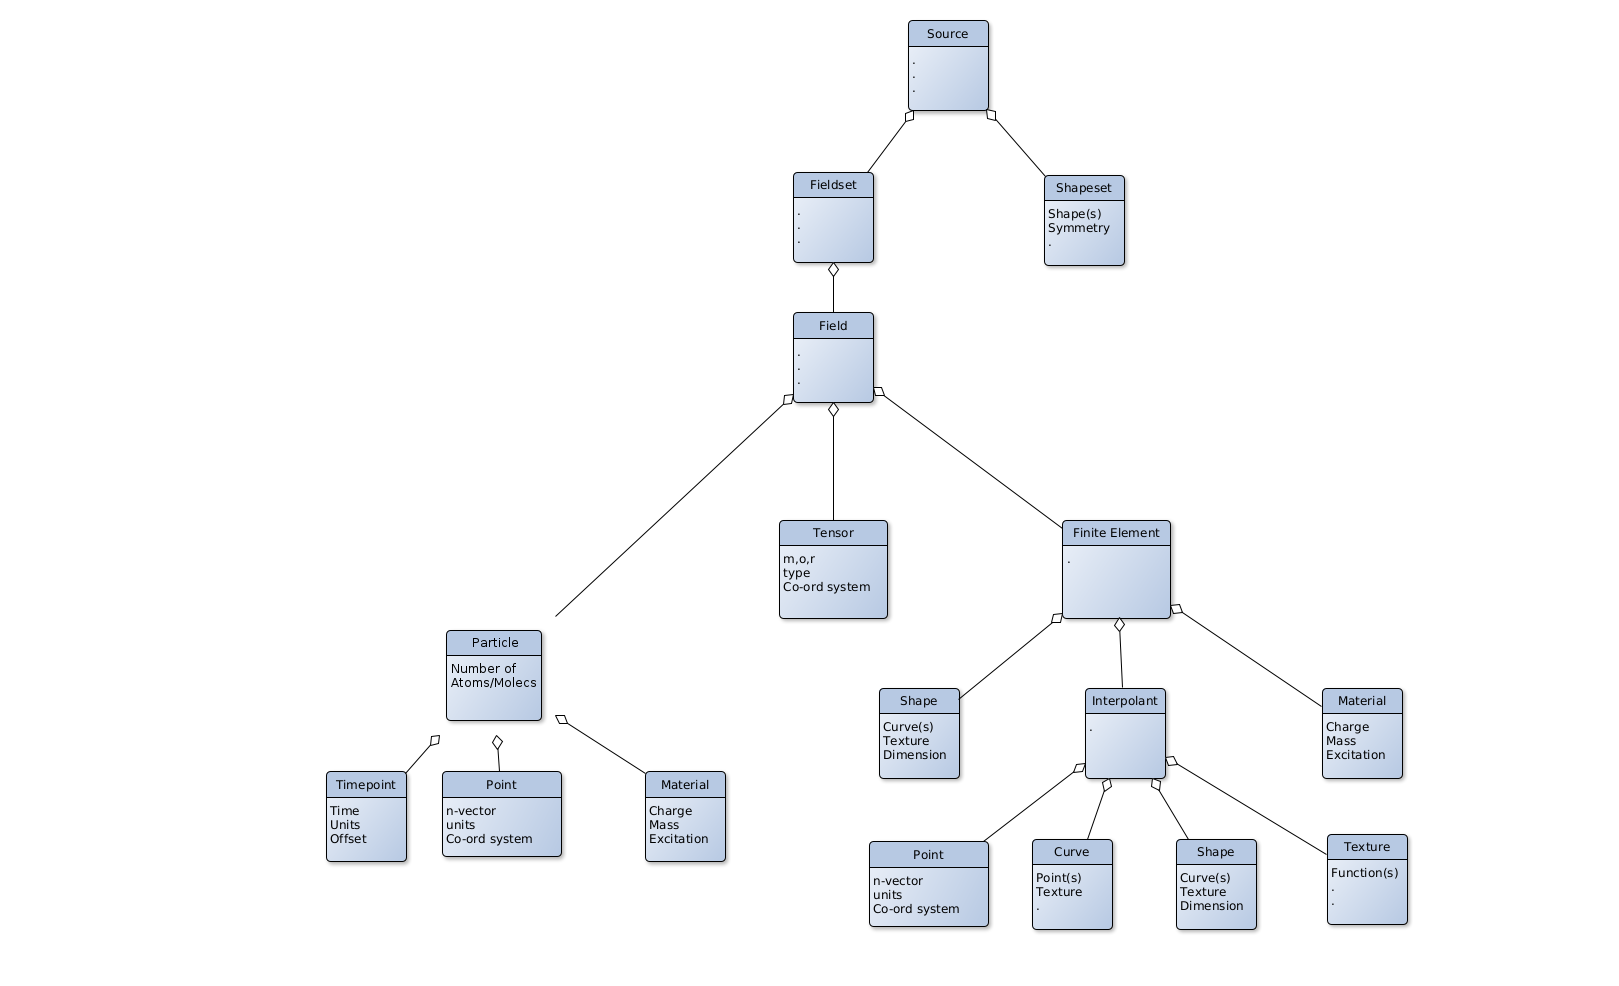
\includegraphics[width=0.7\textwidth]{./pics/aggregates.png}}
\caption{Aggregation of base classes to form a class `Source'.
\label{fig:aggregates}}
\end{figure}
\begin{itemize}
\item
  Particle : parts are location, velocity, material;\\
  Attributes of particle weight
\item
  Interpolant : parts are points, curves, shapes, textures, or
  timepoints, textures
\item
  Diagnostic : parts are DSL input instructions \textbf{Diagnostic
  Processing}, fieldset
\item
  FE (Finite element) : parts are shape, interpolant, material
\item
  Field : parts are tensors and finite elements, or particles;\\
  many make fieldset
\item
  Fieldset : parts are fields
\item
  DE (Differential equation) : parts are operators (DSL input), IC, BC
  and source
\item
  Model : parts are \textbf{Solution of DEs}
\item
  Source : parts are shapeset, fieldset. See \Fig{aggregates}.
\item
  Matexture : parts are materials, textures
\item
  Body : parts are shapeset, matexture
\item
  BC (Boundary Condition) : parts are surface, material, texture
\item
  GEOQ (Geometry plus B-Equil) : parts are shapeset, field
\end{itemize}

\subsection{Simple inherits}\label{sec:simple_inherits}

\begin{itemize}
\item
  HDS (Hierarchical Data Structure) : multi-octree, is a shapeset
\item
  Trajectory : particle position as time varies, is a curve
\item
  IC (Initial Condition) : is a fieldset
\end{itemize}

\subsection{Solution of Differential Equations}\label{sec:solution_of_des}

Use in part ABSTRACT CALCULUS and PUPPETEER patterns (cf.~GoF FACADE)
from Rouson et al. \cite{rousonxiaxu}, see \Sec{desi_patt}.

\subsection{Diagnostic Processing}\label{sec:diagnostic_processing}

\begin{enumerate}
\def\labelenumi{\arabic{enumi}.}
\item
  Read configuration file
\item
  Determine whether any diagnostic needed at present physical time
\item
  Select input fieldset
\item
  Select diagnostic type, use in part ABSTRACT CALCULUS from Rouson et
  al. \cite{rousonxiaxu}

  \begin{itemize}
  \item
    Initial logs

    \begin{itemize}
    \item
      UUID
    \item
      Key input data
    \item
      Key properties, eg. LCFS
    \end{itemize}
  \item
    Combinations of

    \begin{itemize}
    \item
      Field / quadratic field (eg. power, flux quantity) / general
      formula
    \item
      Point, line integral, surface integral, volume integral
    \end{itemize}
  \item
    Mass/charge, momentum/current and power balances
  \item
    Turbulence statistics - cross-correlations, spectra (not particle,
    ray)
  \item
    Difference between solutions/experiment (RMS as `skill') (not
    particle, ray)
  \item
    See ``emergent physics as diagnostic'' in imas\_objects.tex
  \end{itemize}
\item
  Calculate output fieldset
\item
  Set output format
\item
  Output fieldset to disk, screen
\end{enumerate}

\subsection{Orchestration}\label{sec:orchestration}

\begin{enumerate}
\def\labelenumi{\arabic{enumi}.}
\item
  UQ Framework VECMAtk and Fab\nep
\item
  GUI
\item
  CLI
\item
  Possible restart (OLYMPUS logic, Fig.1 of \cite{y2re312})
\item
  \textbf{Initialise} from functions.md
\item
  \textbf{Solution} from functions.md
\end{enumerate}
